\section{Les fonctions d'activations}
Les fonctions d'activation permettent une classification non linéaire. Voici des exemples de fonctions d'activation :
\begin{figure}[htbp!]
    \begin{subfigure}[]{0.32\textwidth}
        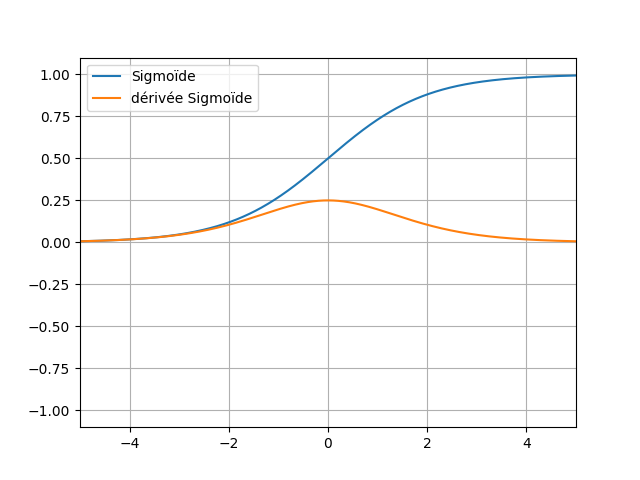
\includegraphics[width=\textwidth]{0-Sigmoide.png}
        \caption{Sigmoïde}
    \end{subfigure}
    \begin{subfigure}[]{0.32\textwidth}
        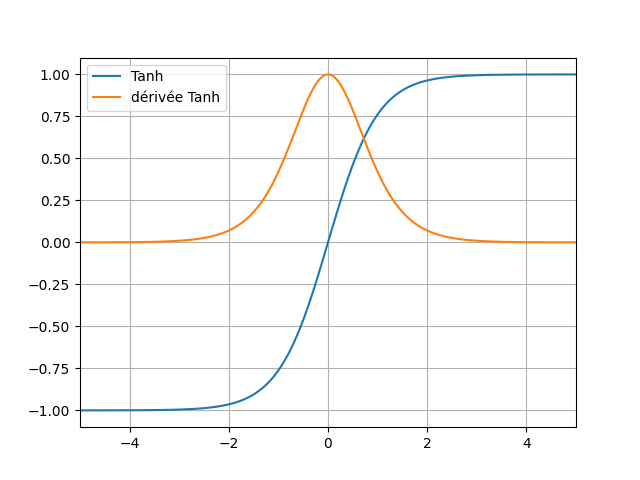
\includegraphics[width=\textwidth]{0-Tanh.png}
        \caption{Tanh}
    \end{subfigure}
    \begin{subfigure}[]{0.32\textwidth}
        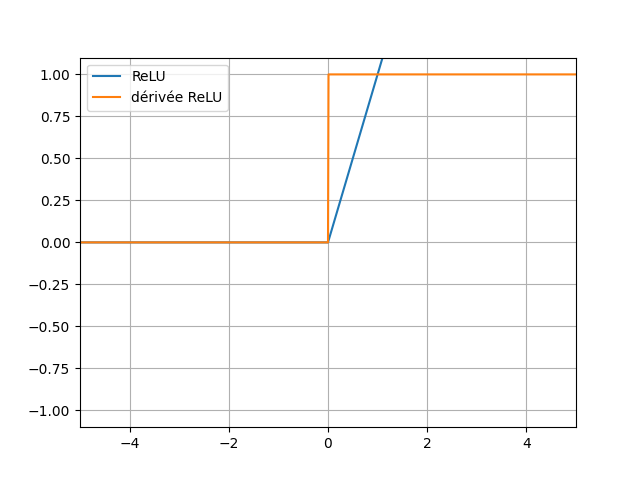
\includegraphics[width=\textwidth]{0-ReLU.png}
        \caption{ReLU}
    \end{subfigure}
\end{figure}
\begin{center}
    \centering
    \begin{tabular}{ l || c | c | }
        Fonction                            & Formule                                          & Dérivée                                    \\ \hline \\
        Sigmoïde (a)                        & $\mathlarger{\frac{1}{1+e^{-x}}}$                & $f(x) \times (1-f(x))$                     \\ \\
        Tangente Hyperbolique (Tanh) (b)    & $\mathlarger{\frac{e^{x}-e^{-x}}{e^{x}+e^{-x}}}$ & $1-f(x)^2$                                 \\ \\
        Unité Linéaire Rectifiée (ReLU) (c) & $max(0, x)$                                      & $ \left\{\begin{array}{ll}
                0 & \mbox{si } x<0 \\
                1 & \mbox{sinon }\end{array}\right.$ \\
    \end{tabular}
\end{center}